\chapter{应用层}

\section{应用层协议}

\subsection{网络应用}

网络应用程序是指能够运行在不同端系统并通过网络彼此通信的程序。例如在Web应用程序中,有两个互相通信的程序,一个是运行在用户主机上的浏览器程序,另一个是运行在Web服务器主机上的服务器程序。\\

应用程序体系结构包括Client-Server和P2P(Peer-to-Peer)两种体系结构。在Client-Server中,服务器主机一直运行处理客户端的请求。因为服务器需要有一个固定的的IP地址,因此客户端能够通过IP地址发送分组与其联系。著名的Client-Server应用程序包括Web、FTP、Telnet和电子邮件等。在Client-Server应用中,经常会出现一台单独的服务器主机不堪重负,跟不上所有客户请求的情况。例如搜索引擎(如Google、Bing、Baidu)、电商(如Amazon、eBay、Alibaba)、电子邮件(如Gmail、Yahoo!)、社交媒体(如Facebook、Instagram、Twitter、WeChat)都分步了多个数据中心,每数据中心都有数十万台服务器,必须要持续供电和维护。而在P2P中,主机之间的通信不必通过专门的服务器,很多流量密集型的应用都是P2P体系结构的,包括对等方协助下载加速器(如迅雷)、文件共享(如BitTorrent)。\\

\subsection{进程通信}

在同一个端系统中,多个进程可以通过进程间通信的机制相互通信,然而在不同的端系统(可能有不同的操作系统)中,需要通过网络交换报文(message)。进程通过套接字(socket)接口向网络发送或接收报文。\\

\begin{figure}[H]
    \centering
    \begin{tikzpicture}
        \draw (0,0) rectangle (3,9);
        \draw (8,0) rectangle (11,9);
        \draw (0,1) -- (3,1);
        \draw (0,2) -- (3,2);
        \draw (0,3) -- (3,3);
        \draw (0,4) -- (3,4);
        \draw (0,5) -- (3,5);
        \draw (0,6.5) -- (3,6.5);
        \draw (8,1) -- (11,1);
        \draw (8,2) -- (11,2);
        \draw (8,3) -- (11,3);
        \draw (8,4) -- (11,4);
        \draw (8,5) -- (11,5);
        \draw (8,6.5) -- (11,6.5);

        \draw (1.5,8.5) node{应用层};
        \draw (1.5,5.5) node{表示层};
        \draw (1.5,4.5) node{会话层};
        \draw (1.5,3.5) node{传输层};
        \draw (1.5,2.5) node{网络层};
        \draw (1.5,1.5) node{数据链路层};
        \draw (1.5,0.5) node{物理层};
        \draw (9.5,8.5) node{应用层};
        \draw (9.5,5.5) node{表示层};
        \draw (9.5,4.5) node{会话层};
        \draw (9.5,3.5) node{传输层};
        \draw (9.5,2.5) node{网络层};
        \draw (9.5,1.5) node{数据链路层};
        \draw (9.5,0.5) node{物理层};

        \draw (1.5,7.5) ellipse (1 and 0.5);
        \draw (9.5,7.5) ellipse (1 and 0.5);
        \draw (1.5,7.5) node{进程};
        \draw (9.5,7.5) node{进程};

        \draw[orange, very thick] (0.75,6) rectangle (2.25,6.75);
        \draw[orange, very thick] (1.5,6.25) node{socket};
        \draw[orange, very thick] (8.75,6) rectangle (10.25,6.75);
        \draw[orange, very thick] (9.5,6.25) node{socket};

        \draw[->, very thick] (-1,9) -- (-1,0);
        \draw[->, very thick] (12,0) -- (12,9);
        \draw[->] (1.5,0) -- (1.5,-1) -- (9.5,-1) -- (9.5,0);
    \end{tikzpicture}
    \caption{socket}
\end{figure}

\vspace{0.5cm}

在进程发送分组的过程中,必须要标识IP地址和端口号(port number)才能将分组发送给另一主机的进程。其中IP地址用于标识主机,端口号用于指定运行在目的主机上的接收进程。由于一台主机上会运行多个应用程序,因此端口号是不可或缺的信息。一些著名的应用已经被分配了特定的端口号,例如Web服务器使用端口号80、邮件服务器(SMTP协议)进程使用端口号25。\\

发送端在使用socket时必须选择一种传输层协议,不同的协议会提供不同的服务。\\

一个传输层协议可以通过四个方面进行分类:

\begin{enumerate}
    \item 可靠数据传输(reliable data transfer):分组在网络传输中可能会因溢出或损坏等原因丢失,对于电子邮件、文件传输和金融相关的应用来说,数据丢失会造成灾难性的后果,这种情况下就必须采用可靠数据传输。对于一些可以容忍丢失(loss-tolerant)的应用,例如多媒体音视频,它们能够承受一定量的数据丢失,这只会造成小干扰,而非致命性的问题。

    \item 吞吐量(throughput):传输层协议能够以特定的速率提供服务。

    \item 定时(timing):传输层协议提供定时保证。例如在网络电话或多人游戏中,较长的时间延迟会出现不自然的停顿或失去真实感。

    \item 安全性(security):传输层协议保证数据安全。例如在发送端将数据加密,并在接收端解密数据,以防在传输被中途被窃听。
\end{enumerate}

\begin{table}[H]
    \centering
    \setlength{\tabcolsep}{5mm}{
        \begin{tabular}{|c|c|c|c|}
            \hline
            \textbf{应用} & \textbf{数据丢失} & \textbf{吞吐量}           & \textbf{时间敏感} \\
            \hline
            文件传输      & 不允许丢失        & 弹性                      & 不                \\
            \hline
            电子邮件      & 不允许丢失        & 弹性                      & 不                \\
            \hline
            网络电话      & 容忍丢失          & few kbps $ \sim $ 1 Mbps  & 100 ms            \\
            \hline
            视频会议      & 容忍丢失          & 10 kbps $ \sim $ 5 Mbps   & 100 ms            \\
            \hline
            交互式游戏    & 容忍丢失          & few kbps $ \sim $ 10 kbps & 100 ms            \\
            \hline
        \end{tabular}
    }
    \caption{常见应用传输服务需求}
\end{table}

\vspace{0.5cm}

\subsection{TCP / UDP}

TCP (Transmission Control Protocol)的特点包括:

\begin{itemize}
    \item 面向连接服务(connection-oriented service):在应用层数据包开始发送之前,TCP让客户端和服务器之间互相交换传输层控制信息,让它们为分组的到来做好准备。在此之后,两个进程的socket就能建立起TCP连接,并可以发送报文了。在发送结束后,该TCP连接会被拆除。

    \item 可靠数据传输:TCP确保了通信进程交付的数据无差错、不丢失、不重复、不乱序。

    \item 拥塞控制(congestion control)
\end{itemize}

UDP(User Datagram Protocol)的特点包括:

\begin{itemize}
    \item 无连接(connectionless)

    \item 不可靠数据传输:UDP不保证报文能够到达接收端,同时报文也有可能是乱序到达的。

    \item 无拥塞控制
\end{itemize}

\begin{table}[H]
    \centering
    \setlength{\tabcolsep}{5mm}{
        \begin{tabular}{|c|c|}
            \hline
            \textbf{应用} & \textbf{传输协议} \\
            \hline
            文件传输      & TCP               \\
            \hline
            电子邮件      & TCP               \\
            \hline
            网络电话      & UDP               \\
            \hline
            视频会议      & UDP               \\
            \hline
            交互式游戏    & UDP               \\
            \hline
        \end{tabular}
    }
    \caption{常见应用传输协议}
\end{table}

\newpage

\section{HTTP}

\subsection{HTTP (HyperText Transfer Protocol)}

一个Web页面是由对象(object)组成的,一个对象就是一个文件,例如HTML文件、JPEG图片、JavaScript文件、CSS样式文件等。如果一个Web页面包含1个HTML文件和5个JPEG图片,那么这个Web页面就有6个对象。\\

每一个对象都可以通过URL(Uniform Resource Locator)寻址,URL地址由存放对象的服务器主机名(host name)和路径名(path name)组成。例如对于http://www.someSchool.edu/someDepartment/picture.gif而言,其中主机名就是www.someSchool.edu,路径名是/someDepartment/picture.gif。\\

HTTP定义在RFC 1945、RFC 7230和RFC 7540中。HTTP使用TCP作为它的支撑传输协议,客户端首先发起TCP连接,连接建立后,客户进程可以向服务器进程发送HTTP请求报文,服务器进程可以向客户进程发送HTTP响应报文。\\

HTTP是一个无状态协议(stateless protocol),服务器不能存储任何关于客户的状态信息。例如某个客户在短时间内两次请求同一个对象,服务器并不会因为第一次已经向客户提供了该对象而不再作出响应,而是再次重新发送对象。\\

\subsection{HTTP请求报文}

HTTP请求报文由第一行的请求行(request line)和后续的首部行(header line)组成,每行由一个回车(carriage return)和换行(line feed)结束,在首部行之后再附加一个只包含回车换行的空行 。\\

\mybox{HTTP请求报文}

\begin{lstlisting}
GET /somedir/page.html HTTP/1.1\r\n
Host: www.someschool.edu\r\n
Connection: close\r\n
User-agent: Mozilla/5.0\r\n
Accept-language: fr\r\n
\r\n
[entity body]
\end{lstlisting}

请求行包含3个字段:

\begin{itemize}
    \item 方法:包括GET、POST、HEAD、PUT和DELETE。

    \item URL:带有请求对象的标识。

    \item HTTP版本
\end{itemize}

首部行中Host指明了对象所在的主机。Connection: close表示浏览器告诉服务器不要使用持续连接,而是要求服务器在发送完对象后就关闭此连接。User-agent指明了用户代理,即向服务器发送请求的浏览器类型,例如Mozilla/5.0。服务器可以通过此信息向用户代理发送不同版本的对象。Accept-language表示用户想要获取对象的语言版本,如果服务器不存在的话,就会发送一个默认版本。\\

使用GET方法时,实体部分(entity body)为空。而使用POST方法时,实体部分可以用于包含用户在表单中填写的输入值。HEAD方法与GET类似,服务器会响应,但并不返回请求对象。因此HEAD方法常用于调试跟踪。PUT方法允许用户向服务器上传对象。DELETE方法允许用户删除服务器上的对象。\\

\subsection{HTTP响应报文}

HTTP响应报文由状态行(status line)、首部行(header line)和实体部分组成。\\

\mybox{HTTP响应报文}

\begin{lstlisting}
HTTP/1.1 200 OK\r\n
Connection: close\r\n
Date: Tue, 18 Aug 2015 15:44:04 GMT\r\n
Server: Apache/2.2.3 (CentOS)\r\n
Last-Modified: Tue, 18 Aug 2015 15:11:03 GMT\r\n
Content-Length: 6821\r\n
Content-Type: text/html\r\n
\r\n
(data data data data data ...)
\end{lstlisting}

状态行包括了协议版本、状态码和对应状态信息。首部行中Connection: close用于告诉客户,发送完报文后将会关闭TCP连接。Date用于表示服务器生成并发送该报文的日期时间。Last-Modified用于表示对象创建或最后修改的日期时间。Content-Length用于表示被发送对象的字节数。Content-Type用于表示对象的类型。\\

\begin{table}[H]
    \centering
    \setlength{\tabcolsep}{5mm}{
        \begin{tabular}{|l|l|}
            \hline
            \textbf{状态码}                & \textbf{含义}                        \\
            \hline
            200 OK                         & 请求成功                             \\
            \hline
            204 No Content                 & 无内容                               \\
            \hline
            301 Moved Permanently          & 永久性重定向,资源被分配了新URL      \\
            \hline
            400 Bad Request                & 请求语法错误,服务器无法理解         \\
            \hline
            403 Forbidden                  & 拒绝执行请求                         \\
            \hline
            404 Not Found                  & 无法找到资源                         \\
            \hline
            500 Internal Server Error      & 服务器内部错误                       \\
            \hline
            503 Service Unavailable        & 由于超载或系统维护,暂时无法处理请求 \\
            \hline
            505 HTTP Version not supported & 不支持请求的HTTP协议的版本           \\
            \hline
        \end{tabular}
    }
    \caption{常见HTTP状态码}
\end{table}

\newpage

\section{Cookie}

\subsection{Cookie}

HTTP服务器是无状态的,然而一些Web站点通常希望能够识别用户,从而记住用户信息或限制用户访问。目前Cookie广泛用于记录用户登录信息,这样下次访问时可以不再输入用户名和密码了。当然这种方便也存在用户信息泄密的问题,尤其在多个用户公用一台电脑时很容易出现这样的情况。\\

\begin{figure}[H]
    \centering
    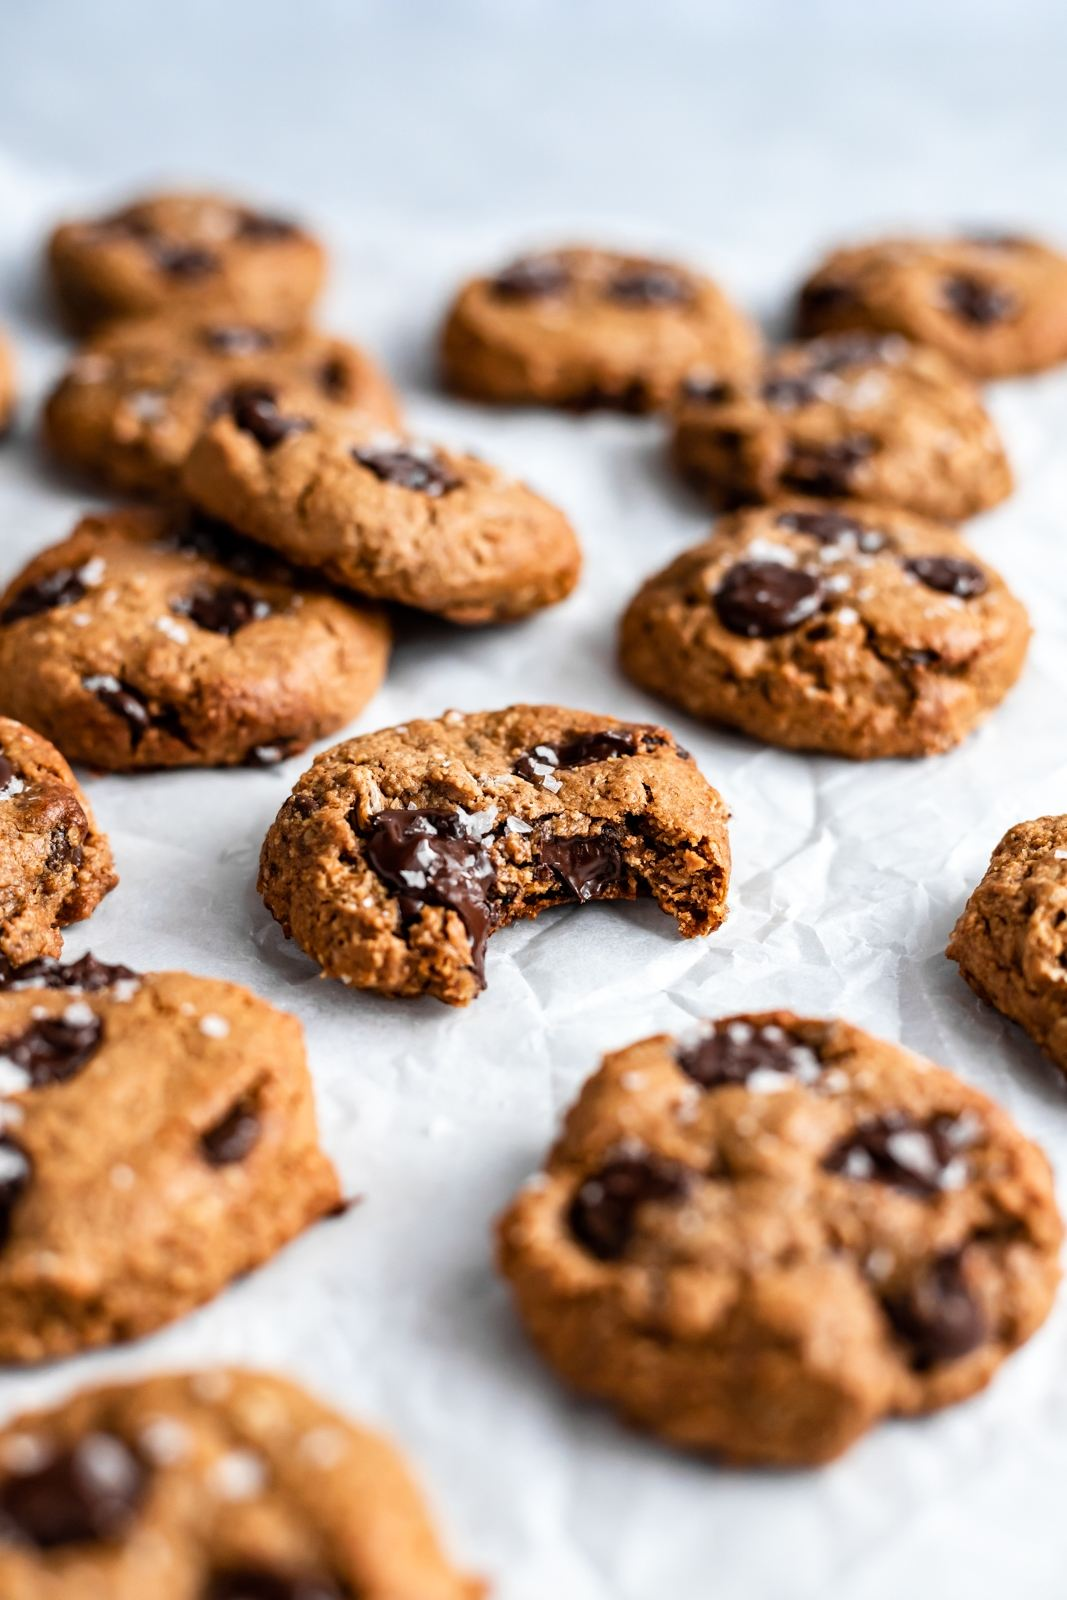
\includegraphics[scale=0.15]{img/Chapter2/2-3/1.png}
\end{figure}

例如用户首次访问Amazon,HTTP响应报文中会包含Set-cookies识别码,浏览器会将识别码添加到所管理的文件中。当用户继续浏览Amazon时,每一个HTTP请求浏览器都会从cookie文件中查询该网站的识别码,并添加到HTTP请求报文中。Amazon也可以通过cookie来维护用户希望购买的商品信息,并推荐个性化产品。

\begin{figure}[H]
    \centering
    \begin{tikzpicture}
        \node at (0,15) {Client};
        \node at (8,15) {Server};

        \draw[loosely dashed, <-] (0,0) -- (0,14);
        \draw[loosely dashed, <-] (8,0) -- (8,14);

        \draw[blue, ->, thick] (0,14) -- (8,12) node[above, midway, sloped]{HTTP request};
        \draw[blue, ->, thick] (8,12) -- (0,10) node[above, midway, sloped]{HTTP response (Set-cookie: 1678)};
        \draw[blue, ->, thick] (0,10) -- (8,8) node[above, midway, sloped]{HTTP request (cookie: 1678)};
        \draw[blue, ->, thick] (8,8) -- (0,6) node[above, midway, sloped]{HTTP response};
        \draw[blue, ->, thick] (0,5) -- (8,3) node[above, midway, sloped]{HTTP request (cookie: 1678)};
        \draw[blue, ->, thick] (8,3) -- (0,1) node[above, midway, sloped]{HTTP response};

        \node at (-2,14) [cylinder, shape border rotate=90, draw, minimum height=12mm, minimum width=10mm] {};
        \node at (-2,13) {eBay: 8734};

        \node at (-2,10) [cylinder, shape border rotate=90, draw, minimum height=12mm, minimum width=10mm] {};
        \node at (-2,9) {eBay: 8734};
        \node at (-2,8.5) {Amazon: 1678};

        \node at (-2,5) [cylinder, shape border rotate=90, draw, minimum height=12mm, minimum width=10mm] {};
        \node at (-2,4) {eBay: 8734};
        \node at (-2,3.5) {Amazon: 1678};

        \node at (11,7) [cylinder, shape border rotate=90, draw, minimum height=12mm, minimum width=10mm] {};
        \node at (11,6) {database};

        \draw[dotted, ->, thick] (8,12) -- (11,7.7) node[above, midway, sloped]{creates ID 1678};
        \draw[dotted, ->, thick] (8,8) -- (10.5,7.5) node[above, midway, sloped]{access};
        \draw[dotted, ->, thick] (8,3) -- (10.5,7) node[above, midway, sloped]{access};
    \end{tikzpicture}
    \caption{Cookie}
\end{figure}

\newpage

\section{Email}

\subsection{SMTP(Simple Mail Transfer Protocol)}

电子邮件系统由用户代理(user agent)、邮件服务器(mail server)和SMTP组成,其中例如Outlook、Apple Mail、Gmail就是用户代理。当Alice发送邮件时,她的用户代理就会向邮件服务器发送邮件,此时邮件被放在邮件服务器的待发报文队列中。当Bob要查看邮件时,他的用户代理就会其邮件服务器中获取该报文。\\

\begin{figure}[H]
    \centering
    \begin{tikzpicture}
        \draw (0,0) rectangle (2.5,2);
        \node at (1.25,1.25) {Alice's};
        \node at (1.25,0.75) {User Agent};

        \draw (4,0) rectangle (6.5,2.5);
        \node at (5.25,2) {Alice's};
        \node at (5.25,1.5) {Mail Server};
        \draw (4.5,0.75) rectangle (6,1);
        \draw (4.3,0.25) rectangle (4.5,0.5);
        \draw (4.7,0.25) rectangle (4.9,0.5);
        \draw (5.1,0.25) rectangle (5.3,0.5);
        \draw (5.5,0.25) rectangle (5.7,0.5);
        \draw (5.9,0.25) rectangle (6.1,0.5);

        \draw (8,0) rectangle (10.5,2.5);
        \node at (9.25,2) {Bob's};
        \node at (9.25,1.5) {Mail Server};
        \draw (8.5,0.75) rectangle (10,1);
        \draw (8.3,0.25) rectangle (8.5,0.5);
        \draw (8.7,0.25) rectangle (8.9,0.5);
        \draw (9.1,0.25) rectangle (9.3,0.5);
        \draw (9.5,0.25) rectangle (9.7,0.5);
        \draw (9.9,0.25) rectangle (10.1,0.5);

        \draw (12,0) rectangle (14.5,2);
        \node at (13.25,1.25) {Bob's};
        \node at (13.25,0.75) {User Agent};

        \draw[->, thick] (2.5,1) -- (4.5,1);
        \draw[->, thick] (6,1) -- (8.25,0.5);
        \draw[->, thick] (10,0.5) -- (12,1);
    \end{tikzpicture}
    \caption{SMTP}
\end{figure}

SMTP是电子邮件中使用的应用层协议,它使用TCP可靠数据传输服务,使用25号端口。\\

SMTP使用命令和应答对报文进行传输:\\

\begin{table}[H]
    \centering
    \setlength{\tabcolsep}{5mm}{
        \begin{tabular}{|c|l|}
            \hline
            \textbf{命令} & \textbf{描述}        \\
            \hline
            HELO          & 与服务器确认信息     \\
            \hline
            AUTH          & 登录验证             \\
            \hline
            MAIL FROM     & 发件人信息           \\
            \hline
            RCPT TO       & 收信人地址           \\
            \hline
            DATA          & 输入邮件基本信息     \\
            \hline
            FROM          & 发信人显示信息       \\
            \hline
            TO            & 服务器收件人显示信息 \\
            \hline
            SUBJECT       & 邮件标题             \\
            \hline
            QUIT          & 断开链接             \\
            \hline
        \end{tabular}
    }
    \caption{SMTP命令}
\end{table}

\begin{table}[H]
    \centering
    \setlength{\tabcolsep}{5mm}{
        \begin{tabular}{|c|l|}
            \hline
            \textbf{返回码} & \textbf{含义}    \\
            \hline
            220             & 服务就绪         \\
            \hline
            250             & 请求动作成功完成 \\
            \hline
            235             & 认证通过         \\
            \hline
            221             & 处理中           \\
            \hline
            354             & 发送开始         \\
            \hline
            500             & 指令错误         \\
            \hline
            550             & 命令无法执行     \\
            \hline
        \end{tabular}
    }
    \caption{SMTP应答返回码}
\end{table}

\vspace{0.5cm}

当用户调用用户代理查看邮件报文时就需要用到邮件访问协议。流行的邮件访问协议有邮局协议版本3(POP3)、因特网邮件访问协议(IMAP, Internet Mail Access Protocol)和HTTP。

\newpage

\section{DNS}

\subsection{DNS(Domain Name System)}

人类可以用很多种方式来表示,比如姓名、身份证号、社保号等,但是人类会更乐意使用容易记忆的姓名而不是社保号。想象一下人们之间这样说话:“你好,我叫132-67-9875”。\\

主机可以使用主机名(hostname)进行表示,例如www.google.com、www.facebook.com,这些名字便于记忆。同时主机也可以使用IP地址进行标识,一个IP地址由4个取值在0 $ \sim $ 255的字节组成,通常以点分十进制表示,如121.7.106.83。\\

路由器更喜欢定长的、有层次结构的IP地址来标记主机,因此域名系统DNS的作用就是进行主机名到IP地址的转换。\\

类似电话本的原理,每一个名字都对应了一个单独的电话号码。DNS最简单的设计就是只使用一个DNS服务器,其中包含所有的映射(mapping),客户端可直接将查询发往该DNS服务器。\\

这种集中式的设计存在几个问题:

\begin{itemize}
    \item 单点故障(single point of failure):如果该DNS服务器故障,整个因特网随之瘫痪。

    \item 通信容量(traffic volume):单个DNS需要处理所有DNS查询。

    \item 远距离集中式数据库(distant centralized database):单个DNS不可能与所有的客户端都相邻,一些地区需要跨越半个地球,造成严重的时延。

    \item 维护(maintainance):中央数据库庞大,需要频繁为新添加的主机更新记录。
\end{itemize}

\vspace{0.5cm}

\subsection{分布式层次数据库}

为了处理扩展性的问题,DNS使用了大量的DNS服务器分布在全世界,并以层次方式组织。\\

DNS服务器分层3类:

\begin{enumerate}
    \item 根DNS服务器
    \item 顶级域(TLD, Top-Level Domain)DNS服务器
    \item 权威(authoritative)DNS服务器
\end{enumerate}

\begin{figure}[H]
    \centering
    \begin{tikzpicture}[
            level distance=2cm,
            level 1/.style={sibling distance=4cm},
            level 2/.style={sibling distance=3cm},
            level 3/.style={sibling distance=2cm}
        ]
        \node {root}
        child {
                node {com}
                child {node {facebook.com}}
                child {node {amazon.com}}
            }
        child {
                node {org}
                child {node {pbs.org}}
            }
        child {
                node {edu}
                child {node {nyu.edu}}
                child {node {umass.edu}}
            };
    \end{tikzpicture}
    \caption{DNS服务器}
\end{figure}

\vspace{0.5cm}

例如一个DNS客户需要获取www.amazon.com的IP地址。客户首先与根服务器之一联系,它将返回顶级域名com的TLD服务器的IP地址。接着客户与TLD服务器之一联系,它将为amazon.com返回权威服务器的IP地址。最后客户与权威服务器之一联系,它将为www.amazon.com返回IP地址。\\

每个ISP都有一个本地DNS服务器(local DNS server),它并不严格属于DNS的层级体系。当主机进行DNS查询时,查询会被发送到本地DNS服务器,再由该本地DNS服务器作为代理(proxy),将查询转发给层级DNS服务器。\\

\begin{figure}[H]
    \centering
    \begin{tikzpicture}
        \draw (0,0) rectangle (2,1);
        \node at (1,0.5) {Host};
        \draw (-1,3) rectangle (3,4);
        \node at (1,3.5) {Local DNS server};
        \draw (5,6) rectangle (9,7);
        \node at (7,6.5) {root DNS server};
        \draw (5,3) rectangle (9,4);
        \node at (7,3.5) {TLD DNS server};
        \draw (5,0) rectangle (10,1);
        \node at (7.5,0.5) {authoritative DNS server};

        \draw[->, blue, thick] (0.75,1) node[above, xshift=-0.2cm]{1} -- (0.75,3);
        \draw[->, blue, thick] (0.75,4) node[above, xshift=-0.2cm]{2} -- (5,6.75);
        \draw[->, blue, thick] (6.75,6) node[below, xshift=-0.2cm]{3} -- (6.75,4);
        \draw[->, blue, thick] (6.75,3) node[below, xshift=-0.2cm]{4} -- (6.75,1);
        \draw[->, blue, thick] (7.25,1) node[above, xshift=0.2cm]{5} -- (7.25,3);
        \draw[->, blue, thick] (7.25,4) node[above, xshift=0.2cm]{6} -- (7.25,6);
        \draw[->, blue, thick] (5,6.25) node[below, xshift=-0.2cm, yshift=-0.2cm]{7} -- (1.25,4);
        \draw[->, blue, thick] (1.25,3) node[below, xshift=0.2cm]{8} -- (1.25,1);
    \end{tikzpicture}
    \caption{DNS递归查询}
\end{figure}

\vspace{0.5cm}

\begin{figure}[H]
    \centering
    \begin{tikzpicture}
        \draw (0,0) rectangle (2,1);
        \node at (1,0.5) {Host};
        \draw (-1,3) rectangle (3,4);
        \node at (1,3.5) {Local DNS server};
        \draw (5,6) rectangle (9,7);
        \node at (7,6.5) {root DNS server};
        \draw (5,3) rectangle (9,4);
        \node at (7,3.5) {TLD DNS server};
        \draw (5,0) rectangle (10,1);
        \node at (7.5,0.5) {authoritative DNS server};

        \draw[->, blue, thick] (0.75,1) node[above, xshift=-0.2cm]{1} -- (0.75,3);
        \draw[->, blue, thick] (0.75,4) node[above, xshift=-0.2cm]{2} -- (5,6.75);
        \draw[->, blue, thick] (5,6.25) node[below, xshift=-0.2cm, yshift=-0.2cm]{3} -- (1.25,4);
        \draw[->, blue, thick] (3,3.75) node[above, xshift=0.2cm]{4} -- (5,3.75);
        \draw[->, blue, thick] (5,3.25) node[below, xshift=-0.2cm]{5} -- (3,3.25);
        \draw[->, blue, thick] (2.5,3) node[right, xshift=0.5cm, yshift=-0.2cm]{6} -- (6,1);
        \draw[->, blue, thick] (5.5,1) node[left, xshift=-0.5cm]{7} -- (2,3);
        \draw[->, blue, thick] (1.25,3) node[below, xshift=0.2cm]{8} -- (1.25,1);
    \end{tikzpicture}
    \caption{DNS迭代查询}
\end{figure}

为了减少时延并减少传输DNS报文的数量,DNS使用了DNS缓存(DNS caching)。只要DNS服务器获得了IP映射,就将其缓存,因此根DNS服务器不会再被经常访问。然而IP映射并不是永久的,DNS服务器在一段时间后将会丢弃缓存信息。

\newpage

\section{P2P}

\subsection{P2P(Peer-to-Peer)}

P2P体系结构中,其中每个peer节点都能够帮助服务器来分发文件。也就是说,当一个peer节点接收到文件数据时,它可以利用自己的上载能力重新将数据分发给其它peer节点。\\

\begin{figure}[H]
    \centering
    \begin{tikzpicture}
        \draw (0,0) rectangle (2,1);
        \node at (1,0.5) {Server};
        \node at (-1,0.5) [cylinder, shape border rotate=90, draw, minimum height=12mm, minimum width=10mm] {F};

        \draw (4,3) rectangle (6,4);
        \node at (5,3.5) {peer};
        \draw (8,3) rectangle (10,4);
        \node at (9,3.5) {peer};
        \draw (5,-3) rectangle (7,-4);
        \node at (6,-3.5) {peer};

        \draw (5,-1) rectangle (9,1);
        \node at (7,0) {Internet};

        \draw[->, thick] (2,0.5) node[right, yshift=0.2cm]{$ u_s $} -- (5,0);
        \draw[->, thick] (4.5,3) node[left, xshift=0.5cm, yshift=-1cm]{$ u_1 $} -- (6,1);
        \draw[->, thick] (6.5,1) node[right, xshift=-0.5cm, yshift=1cm]{$ d_1 $} -- (5,3);
        \draw[->, thick] (8.5,3) node[left, xshift=-0.5cm, yshift=-1cm]{$ u_2 $} -- (7.5,1);
        \draw[->, thick] (8,1) node[right, xshift=0.5cm, yshift=1cm]{$ d_2 $} -- (9,3);
        \draw[->, thick] (6,-3) node[left, yshift=1cm]{$ u_N $} -- (6.5,-1);
        \draw[->, thick] (7,-1) node[right, yshift=-1cm]{$ d_N $} -- (6.5,-3);
    \end{tikzpicture}
    \caption{P2P}
\end{figure}

\vspace{0.5cm}

\subsection{BitTorrent}

BitTorrent是一种用于文件分发的P2P协议,其中参与一个特定文件分发的所有peer的集合被称为洪流(torrent)。在一个torrent中的peer彼此下载等长度的文件块(chunk),块长度通常为256KB。\\

当一个peer节点一开始加入一个torrent时,它没有文件块。随着时间的推移,它将累积越来越多的文件块。当它下载文件块时,也为其它peer节点上载了多个文件块。peer节点一但获得了整个文件,它可以自私地离开torrent,也可以大公无私地留在torrent中并继续向其它peer节点上载文件块。\\

例如,当一个peer节点Alice加入torrent时,追踪服务器随机选择一些peer节点,并将这些peer节点的IP地址发送给Alice。Alice持有这些peer节点的列表,试着与该列表上的多个peer节点创建并行的TCP连接。这里称所有与Alice成功地创建TCP连接的peer节点为邻近peer节点(neighboring peers)。\\

随着时间的推移,其中的一些peer节点可能离开,而其它peer节点可能试着与Alice创建TCP连接。因此,邻近peer节点会随着时间而改变。\\

在任何时刻,每个peer节点都拥有来自某文件块的子集,且不同的peer节点具有不同的文件块子集。Alice周期性地询问每个邻近peer节点它们所具有的块列表,并对当前还没有的块发出请求。\\

Alice使用一种称为最稀缺优先(rarest first)的策略,其思路是根据她没有的块从她的邻居中找到拷贝数量最少的那些块,并优先请求这些稀缺块。因此,最稀缺的块会更迅速地分发,其目标是均衡每个块在torrent中的拷贝数量。

\newpage

\section{视频流}

\subsection{视频流(Video Streaming)}

视频是由一系列的图像,以一种恒定的速率(如每秒24张或30张图像)来展现的。一幅未压缩、数字编码的图像由像素阵列(array of pixels)组成,其中每个像素都是由一些比特编码来表示亮度和颜色。\\

视频的一个重要特征就是能够被压缩,因而可用比特率(bit rate)来权衡视频质量。视频有各种各样的压缩算法,对应不同的比特率。视频信息之所以存在大量可以被压缩的空间,是因为其中本身就存在大量的数据冗余。\\

如果分析一个视频里的每一帧,我们会看到有许多区域是相互关联的。因此在传输比特时,可以传输颜色值及其重复次数,而不是传输多个相同的颜色值。\\

\begin{figure}[H]
    \centering
    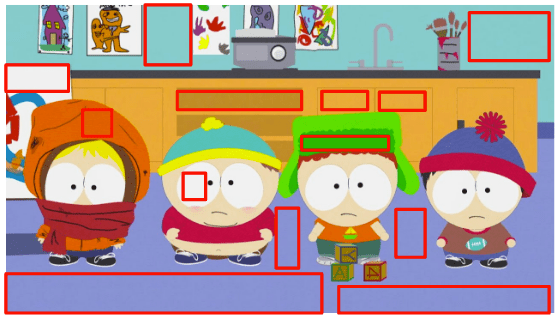
\includegraphics[scale=0.7]{img/Chapter2/2-7/1.png}
    \caption{空间冗余}
\end{figure}

另一种是时间冗余,对于连续的两帧,尝试花费较少的数据量进行编码,只传输两帧之间发生改变的地方,而不用全部传输。\\

\begin{figure}[H]
    \centering
    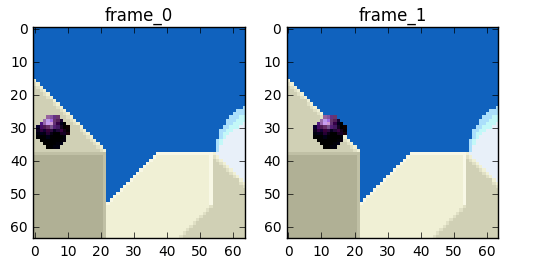
\includegraphics[scale=0.7]{img/Chapter2/2-7/2.png}
    \caption{时间冗余}
\end{figure}

\vspace{0.5cm}

\subsection{DASH(Dynamic Adaptive Streaming over HTTP)}

在HTTP流中,视频只是存储在HTTP服务器中的一个普通文件,每个文件都有一个特定的URL。但是因为如此,所有客户接收到的视频编码版本也相同,显然这并没有考虑用户的带宽问题。\\

DASH,即经HTTP的动态适应流,解决了这个问题。在DASH流中,将视频编码成几个不同的版本,每个版本都具有不同的比特率,每个版本都有属于自己的URL。DASH在初始时能够根据用户的带宽选择一个合适的版本,同时也允许用户自定义更换版本。\\

\subsection{CDN(Content Distribution Network)}

服务器一定都是有物理位置的,因此离服务器越远的地方访问服务器就会越慢。况且很多中小型网站的服务器本身使用的带宽就小,一旦同时访问的人一多,访问网站依然会很慢。另一个问题就是服务器都会有一定几率遇到宕机的问题,服务器出了问题就导致无法打开网站。\\

内容分发网CDN的出现就可以解决这个问题。它与电商的仓库管理方式非常类似,电商刚开始的时候,买家购买一样物品后,商家都只能从仓库所在地发货,所以物流时间需要3$ \sim $10天不等。后来电商和物流公司想了个招,在全国各个区域都建设仓储中心,先把货物放到这些仓储中心,这样买家不管在哪个地方,直接从最近的仓库发货,这样就能减少物流时间。\\

CDN管理分布在多个地理位置上的服务器,在它的服务器上存储视频(包括其它Web内容)的副本,并且将每个用户请求定向到一个能提供最好用户体验的CDN位置。

\newpage

\section{Socket编程}

\subsection{Socket}

Socket(套接字)是对TCP/IP网络协议进行的包装(协议的抽象应用),它本身最大的特点是提供了不同进行之间的数据通讯操作。所有的网络协议的组成是非常繁琐的,如果所有的开发者去研究具体的通讯协议会对开发带来很大的难度,所以在不同的编程语言内部就会考虑对一些网络的协议进行包装。\\

Socket主要是针对两种协议的包装:

\begin{itemize}
    \item 传输控制协议TCP(Transmission Control Protocol):采用有状态的通讯机制进行传输,在通讯时会通过三次握手机制保证与一个指定节点的数据传输的可靠性,在通讯完毕后会通过四次挥手的机制关闭连接。由于在每次数据通讯前都需要消耗大量的时间进行连接控制,所以执行性能较低,且系统资源占用较大。

    \item 用户数据报协议UDP(User Datagram Protocol):采用无状态的通讯机制进行传输,没有了TCP中复杂的握手与挥手处理机制,这样就节约了大量的系统资源,同时数据传输性能较高。但是由于不保存单个节点的连接状态,所以发送的数据不一定可以被全部接收。UDP不需要连接就可以直接发送数据,并且多个接收端都可以接收同样的消息,所以使用UDP适合于广播操作。
\end{itemize}

\vspace{0.5cm}

\subsection{字节序(Endianness)}

字节序是指多字节数据在计算机内存中存储或者网络传输时各字节的存储顺序。计算机有两种储存数据的方式,分别是大端字节序(big endian)和小端字节序(little endian)。\\

例如存储两个十六进制数0x12345678和0x11223344,小端字节序把值的低位存在低地址,而大端字节序把值的高位存在低地址。\\

\begin{figure}[H]
    \centering
    \begin{tikzpicture}[font=\ttfamily,
            array/.style={matrix of nodes,nodes={draw, minimum size=10mm, fill=green!30},column sep=-\pgflinewidth, row sep=0.5mm, nodes in empty cells,
                    row 1/.style={nodes={draw=none, fill=none, minimum size=5mm}},
                }]

        \matrix[array] (array) {
            低   &      &      &      &      &      &      & 高   \\
            0x78 & 0x56 & 0x34 & 0x12 & 0x44 & 0x33 & 0x22 & 0x11 \\
        };
    \end{tikzpicture}
    \caption{小端字节序}
\end{figure}

\begin{figure}[H]
    \centering
    \begin{tikzpicture}[font=\ttfamily,
            array/.style={matrix of nodes,nodes={draw, minimum size=10mm, fill=green!30},column sep=-\pgflinewidth, row sep=0.5mm, nodes in empty cells,
                    row 1/.style={nodes={draw=none, fill=none, minimum size=5mm}},
                }]

        \matrix[array] (array) {
            低   &      &      &      &      &      &      & 高   \\
            0x12 & 0x34 & 0x56 & 0x78 & 0x11 & 0x22 & 0x33 & 0x44 \\
        };
    \end{tikzpicture}
    \caption{大端字节序}
\end{figure}

由此引发了计算机界的大端与小端之争,不同的CPU厂商并没有达成一致。在网络通信中,RFC1700规定使用大端字节序作为网络字节序。因此不使用大端的计算机在发送数据时必须将自己的主机字节序转换为网络字节序,接收数据时需要转换成自己的主机字节序,这样就与CPU和操作系统无关了。\\

htons()和htonl()可用于将主机字节序转换为网络字节序,ntohs()和ntohl()可用于将网络字节序转换为主机字节序。\\

\subsection{TCP}

Socket是在应用层和传输层之间的一个抽象层,它把TCP/IP层复杂的操作抽象为几个简单的接口供应用层调用已实现进程在网络中通信。\\

Socket起源于UNIX一切皆文件的哲学思想,服务器和客户端各自维护一个Socket,在建立连接后,可以向自己Socket写入内容供对方读取或者读取对方内容,通讯结束时关闭Socket。\\

\begin{figure}[H]
    \centering
    \begin{tikzpicture}
        \node at (1,16.5) {服务器};
        \draw (0,15) rectangle (2,16);
        \node at (1,15.5) {socket()};
        \draw (0,13) rectangle (2,14);
        \node at (1,13.5) {bind()};
        \draw (0,11) rectangle (2,12);
        \node at (1,11.5) {listen()};
        \draw (0,9) rectangle (2,10);
        \node at (1,9.5) {accept()};
        \draw (0,5) rectangle (2,6);
        \node at (1,5.5) {read()};
        \draw (0,2) rectangle (2,3);
        \node at (1,2.5) {write()};
        \draw (0,0) rectangle (2,1);
        \node at (1,0.5) {close()};

        \draw[->, thick] (1,15) -- (1,14);
        \draw[->, thick] (1,13) -- (1,12);
        \draw[->, thick] (1,11) -- (1,10);
        \draw[->, thick] (1,9) node[left, yshift=-1.5cm]{阻塞直到收到客户连接} -- (1,6);
        \draw[->, thick] (1,5) node[left, yshift=-1cm]{处理请求} -- (1,3);
        \draw[->, thick] (0,2.5) -- (-1,2.5) -- (-1,5.5) -- (0,5.5);
        \draw[->, thick] (1,2) -- (1,1);

        \node at (9,16.5) {客户端};
        \draw (8,15) rectangle (10,16);
        \node at (9,15.5) {socket()};
        \draw (8,7) rectangle (10,8);
        \node at (9,7.5) {connect()};
        \draw (8,5) rectangle (10,6);
        \node at (9,5.5) {write()};
        \draw (8,2) rectangle (10,3);
        \node at (9,2.5) {read()};
        \draw (8,0) rectangle (10,1);
        \node at (9,0.5) {close()};

        \draw[->, thick] (9,15) -- (9,8);
        \draw[->, thick] (9,7) -- (9,6);
        \draw[->, thick] (9,5) -- (9,3);
        \draw[->, thick] (10,2.5) -- (11,2.5) -- (11,5.5) -- (10,5.5);
        \draw[->, thick] (9,2) -- (9,1);

        \draw[<->, thick] (1,7.5) node[above, xshift=4cm] {建立连接} -- (8,7.5);
        \draw[<->, thick] (2,5.5) node[above, xshift=3cm] {数据请求} -- (8,5.5);
        \draw[<->, thick] (2,2.5) node[above, xshift=3cm] {数据响应} -- (8,2.5);
        \draw[<->, thick] (2,0.5) node[above, xshift=3cm] {关闭连接} -- (8,0.5);
    \end{tikzpicture}
    \caption{TCP}
\end{figure}

\vspace{0.5cm}

\subsubsection{socket()}

\begin{itemize}
    \item IP地址类型:
          \begin{itemize}
              \item AF\_INET(IPv4)
              \item AF\_INET6(IPv6)
          \end{itemize}

    \item 数据传输方式/套接字类型:
          \begin{itemize}
              \item SOCK\_STREAM(流格式套接字/面向连接的套接字)
              \item SOCK\_DGRAM(数据报套接字/无连接的套接字)
          \end{itemize}
\end{itemize}

\vspace{0.5cm}

\subsubsection{bind()}

将Socket和本地地址绑定,地址包括IP和端口号。\\

127.0.0.1用于表示本地地址。\\

端口号的范围为0$ \sim $65535,其中0$ \sim $1023为知名端口(well known ports),用于绑定一些常用服务。\\

\subsubsection{listen()}

监听,将接收到的客户端连接放入队列。\\

\subsubsection{accept()}

从队列获取请求,返回客户端Socket描述符。当已完成连接队列的下一个完成连接是空, 那么accept()将被阻塞。\\

\subsubsection{read() / write()}

双向通信。read()负责从Socket中读取内容,write()负责将内容写入Socket中。\\

\subsubsection{close()}

关闭Socket,终止TCP/UDP连接。\\

\mybox{TCP}

\begin{lstlisting}[language=Python, title=tcp\_server.py]
import socket

SERVER_HOST = "127.0.0.1"
SERVER_PORT = 8080

def main():
    sock = socket.socket(socket.AF_INET, socket.SOCK_STREAM)
    sock.bind((SERVER_HOST, SERVER_PORT))
    sock.listen()
    print("[Server] Server started.")
    print("[Server] Waiting for connection...")

    # Get client's socket and address
    client, client_addr = sock.accept()
    print("[Server] Client%s:%s Connected to server." % client_addr)

    while True:
        data = client.recv(100).decode("UTF8")
        print("[Server] Received: %s" % data)
        if data == "exit":
            client.send("exit".encode("UTF8"))
            break
        else:
            client.send(data.encode("UTF8"))
    
    sock.close()

if __name__ == "__main__":
    main()
\end{lstlisting}

\begin{lstlisting}[language=Python, title=tcp\_client.py]
import socket

SERVER_HOST = "127.0.0.1"
SERVER_PORT = 8080

def main():
    sock = socket.socket(socket.AF_INET, socket.SOCK_STREAM)
    sock.connect((SERVER_HOST, SERVER_PORT))

    while True:     
        msg = input("[Client] Enter data: ")
        sock.send(msg.encode("UTF8"))
        reply = sock.recv(100).decode("UTF8")
        if reply == "exit":
            break
        else:
            print("[Server] " + reply)

    sock.close()

if __name__ == "__main__":
    main()
\end{lstlisting}

\vspace{0.5cm}

\subsection{UDP}

UDP是尽最大能力进行传输,但是并不能保证可靠性,丢包并不会重发。TCP的可靠性是因为一系列的机制保证可靠性。两种协议并没有优略之分,要区分不同的场景来区分。\\

例如进行文件传输,不能有数据丢失,TCP协议就更合适,而进行实时视频通话,UDP会根据恒定的速率进行发送,这样的情况容许部分数据的丢失去追求更好的实时性,所以UDP更合适。\\

\mybox{UDP}

\begin{lstlisting}[language=Python, title=udp\_server.py]
import socket

SERVER_HOST = "127.0.0.1"
SERVER_PORT = 8080

def main():
    sock = socket.socket(socket.AF_INET, socket.SOCK_DGRAM)
    sock.bind((SERVER_HOST, SERVER_PORT))
    print("[Server] Server started.")
    print("[Server] Waiting for connection...")

    while True:
        data, client_addr = sock.recvfrom(100)
        print("[Server] Client%s:%s: " % client_addr, end=":")
        data = data.decode("UTF8")
        print(data)
        if data == "exit":
            sock.sendto("exit".encode("UTF8"))
            break
        else:
            sock.sendto(data.encode("UTF8"), client_addr)
    
    sock.close()

if __name__ == "__main__":
    main()
\end{lstlisting}

\begin{lstlisting}[language=Python, title=udp\_client.py]
import socket

SERVER_HOST = "127.0.0.1"
SERVER_PORT = 8080

def main():
    sock = socket.socket(socket.AF_INET, socket.SOCK_DGRAM)

    while True:     
        msg = input("[Client] Enter data: ")
        sock.sendto(msg.encode("UTF8"), (SERVER_HOST, SERVER_PORT))
        reply, addr = sock.recvfrom(100)
        reply = reply.decode("UTF8")
        if reply == "exit":
            break
        else:
            print("[Server] " + reply)

    sock.close()

if __name__ == "__main__":
    main()
\end{lstlisting}

\newpage